% =====================================================================
% 附录 C：补充实验。由原 appendix.tex（A.6--A.10）与
% appendix_additional.tex（B.2--B.6）搬运，按主文实验节顺序排列。
% =====================================================================
\section{Additional experiments}
\label{app:experiments}

\subsection{Main results with standard deviations}
\label{app:main-std}

Tables~\ref{tab:main_result_std_baselines} and~\ref{tab:main_result_std_variants}
report the same configurations as the main table with standard deviations over
runs, split by column groups for width (the baselines table includes NCBD and the
variants table includes AdaCap); bold and underline follow the same
mean-based rule as Table~\ref{tab:main_result}.

% 主结果表（带标准差）：由 paper/make_table.py 从 tune_results/*.html 自动生成，请勿手改。
% 因 8 方法列 × (均值±std) 超出页宽，按列拆为两张表：
% (a) baselines（Base/VIB/SVIB/NIB，tab:main_result_std_baselines）；
% (b) CEB/DVCCA 与 GPB/GPB-L（tab:main_result_std_variants，竖线分隔同主表）。
% 每表含全部 12 行；分类 Acc（%）、回归 R²，单元格为均值±std；
% 加粗/下划线按该行全部 8 列的均值判定（与 main_result.tex 一致）；
% 表尾排名行省略（与主表重复）。
\begin{table*}[t]
\centering
\caption{Test accuracy (\%) and test $R^2$ with standard deviations over runs: the plain backbone and the variational baselines; same configurations as Table~\ref{tab:main_result}.}
\label{tab:main_result_std_baselines}
\small
{
\setlength{\tabcolsep}{2pt}
\begin{tabular}{llcccc}
\hline
Dataset & Backbone & Base & VIB & SVIB & NIB \\
\hline
MNIST & MLP & 98.33$\pm$0.12 & 98.28$\pm$0.11 & 98.15$\pm$0.13 & 98.27$\pm$0.07 \\
MNIST & CNN & 99.13$\pm$0.05 & 99.28$\pm$0.09 & 99.23$\pm$0.03 & 99.22$\pm$0.06 \\
ImageNet-100 & MLP & 83.12$\pm$0.14 & 82.84$\pm$0.44 & 83.02$\pm$0.37 & 82.35$\pm$0.27 \\
ImageNet-100 & CNN & 83.40$\pm$0.13 & 82.94$\pm$0.37 & 83.11$\pm$0.86 & 82.91$\pm$0.35 \\
Cora & GCN & 87.68$\pm$0.46 & 86.83$\pm$0.28 & 86.46$\pm$1.87 & 86.35$\pm$0.68 \\
IMDb & RNN & 84.85$\pm$0.68 & 85.50$\pm$0.91 & 85.99$\pm$0.30 & 86.14$\pm$0.92 \\
AG News & RNN & \textbf{92.94$\pm$0.15} & 92.72$\pm$0.17 & 92.86$\pm$0.21 & 92.91$\pm$0.22 \\
\hline\hline
Cal. Housing & MLP & 0.7618$\pm$0.0238 & \underline{0.7901$\pm$0.0049} & 0.7897$\pm$0.0058 & 0.7862$\pm$0.0035 \\
STS-B & RNN & \textbf{0.2899$\pm$0.0113} & 0.2719$\pm$0.0164 & 0.2697$\pm$0.0202 & 0.2417$\pm$0.0221 \\
ZINC & GCN & \textbf{0.6348$\pm$0.0044} & 0.6339$\pm$0.0033 & 0.6325$\pm$0.0026 & 0.6178$\pm$0.0099 \\
AgeDB & MLP & 0.2180$\pm$0.0409 & 0.3173$\pm$0.0101 & \underline{0.3385$\pm$0.0286} & 0.2710$\pm$0.0235 \\
AgeDB & CNN & 0.3914$\pm$0.0194 & 0.3342$\pm$0.1894 & 0.3323$\pm$0.1870 & 0.3337$\pm$0.1889 \\
\hline
\end{tabular}
}
\end{table*}
\par\smallskip
\begin{table*}[t]
\centering
\caption{Test accuracy (\%) and test $R^2$ with standard deviations over runs: CEB, DVCCA, and our method; same configurations as Table~\ref{tab:main_result}. GPB and GPB-L are separated from the references by the vertical rule.}
\label{tab:main_result_std_variants}
\small
{
\setlength{\tabcolsep}{2pt}
\begin{tabular}{llcc|cc}
\hline
Dataset & Backbone & CEB & DVCCA & GPB & GPB-L \\
\hline
MNIST & MLP & \underline{98.43$\pm$0.08} & 98.24$\pm$0.17 & \textbf{98.54$\pm$0.09} & \underline{98.43$\pm$0.07} \\
MNIST & CNN & 99.30$\pm$0.05 & 99.29$\pm$0.10 & \textbf{99.32$\pm$0.05} & \underline{99.31$\pm$0.05} \\
ImageNet-100 & MLP & 82.77$\pm$0.22 & 82.99$\pm$0.43 & \textbf{84.40$\pm$0.21} & \underline{84.01$\pm$0.23} \\
ImageNet-100 & CNN & 82.97$\pm$0.67 & 83.21$\pm$0.70 & \textbf{86.08$\pm$0.21} & \underline{84.88$\pm$0.80} \\
Cora & GCN & 86.27$\pm$0.38 & 86.90$\pm$0.94 & \textbf{88.12$\pm$0.55} & \underline{87.86$\pm$0.87} \\
IMDb & RNN & 85.55$\pm$0.73 & 85.69$\pm$0.23 & \underline{86.84$\pm$0.57} & \textbf{86.99$\pm$0.35} \\
AG News & RNN & 92.83$\pm$0.11 & 92.78$\pm$0.15 & 92.87$\pm$0.12 & \underline{92.92$\pm$0.14} \\
\hline\hline
Cal. Housing & MLP & 0.7894$\pm$0.0018 & 0.7878$\pm$0.0048 & 0.7895$\pm$0.0051 & \textbf{0.7914$\pm$0.0034} \\
STS-B & RNN & 0.2668$\pm$0.0127 & 0.2713$\pm$0.0218 & \underline{0.2762$\pm$0.0152} & 0.2755$\pm$0.0134 \\
ZINC & GCN & 0.6257$\pm$0.0044 & 0.6294$\pm$0.0026 & \underline{0.6344$\pm$0.0031} & 0.6323$\pm$0.0016 \\
AgeDB & MLP & 0.3317$\pm$0.0251 & 0.3180$\pm$0.0228 & \textbf{0.3536$\pm$0.0076} & 0.3320$\pm$0.0080 \\
AgeDB & CNN & 0.3882$\pm$0.0275 & 0.3205$\pm$0.1811 & \textbf{0.4700$\pm$0.0072} & \underline{0.4388$\pm$0.0220} \\
\hline
\end{tabular}
}
\end{table*}
\par\smallskip

\subsection{Paired-difference confidence intervals}
\label{app:main-ci}

Tables~\ref{tab:main_result_ci_baselines}--\ref{tab:main_result_ci_external}
report, for each setting, the paired difference of GPB over every baseline
(GPB minus baseline) with a bootstrap $95\%$ confidence interval: the differences
are paired across the shared seeds, the interval is the percentile interval of
$B = 10{,}000$ resamples of the per-run differences (fixed seed, reproducible), and
the non-inferiority margin is $\delta_{\rm NI} = 0.2$ percentage points of accuracy or
$\delta_{\rm NI} = 0.005$ in $R^2$. Bold marks a lower bound above zero (significant
advantage) and $^{\dagger}$ a lower bound within the margin (tied); the best
configuration per method is the same as in the main table. The last table covers
the external non-IB baselines, NCBD on the classification settings and AdaCap on
the regression settings; the only interval lying entirely below zero is AdaCap on
ZINC ($-0.043$ $R^2$).

% 主结果差值 CI 表：由 paper/make_table.py 从 tune_results 自动生成，请勿手改。
% 行 = 12 个 setting；单元格 = GPB − baseline 的配对差值 [bootstrap 95% CI]
%（分类百分点、回归 R²）；加粗 = CI 下限 > 0（显著更优）、† = CI 下限 > −δ
%（非劣界 δ=0.2 百分点 / 0.005）记 tied；
% 同 seed 配对（run 顺序即 seed 0..N−1），bootstrap B=10000（固定 seed 0，百分位法）。
% 因 7 个差值列超页宽，按列拆两张表（baselines / ceb+dvcca+OPB-L）；表尾一行统计各列 */† 次数。
\begin{table*}[t]
\centering
\caption{Paired-difference 95\% confidence intervals of GPB over the plain backbone and VIB (GPB minus baseline, per setting; classification in percentage points, regression in $R^2$). Bold: lower CI bound above zero; $^{\dagger}$: lower bound within the non-inferiority margin $\delta$ (tied).}
\label{tab:main_result_ci_baselines}
\small
{
\setlength{\tabcolsep}{1pt}
\begin{tabular}{llcc}
\hline
Dataset & Backbone & Base & VIB \\
\hline
MNIST & MLP & \textbf{+0.2 [+0.2, +0.3]} & \textbf{+0.3 [+0.2, +0.3]} \\
MNIST & CNN & \textbf{+0.2 [+0.2, +0.2]} & +0.0 [-0.0, +0.1]$^{\dagger}$ \\
ImageNet-100 & MLP & \textbf{+1.3 [+1.2, +1.4]} & \textbf{+1.6 [+1.4, +1.9]} \\
ImageNet-100 & CNN & \textbf{+2.7 [+2.5, +2.9]} & \textbf{+3.1 [+3.0, +3.4]} \\
Cora & GCN & +0.4 [-0.1, +1.1]$^{\dagger}$ & \textbf{+1.3 [+0.7, +1.7]} \\
IMDb & RNN & \textbf{+2.0 [+1.2, +2.7]} & \textbf{+1.3 [+0.6, +2.3]} \\
AG News & RNN & -0.1 [-0.2, +0.0]$^{\dagger}$ & \textbf{+0.2 [+0.1, +0.2]} \\
\hline\hline
Cal. Housing & MLP & \textbf{+0.028 [+0.008, +0.048]} & -0.001 [-0.005, +0.003]$^{\dagger}$ \\
STS-B & RNN & -0.014 [-0.022, -0.006] & +0.004 [-0.017, +0.022] \\
ZINC & GCN & -0.000 [-0.003, +0.002]$^{\dagger}$ & +0.001 [-0.004, +0.004]$^{\dagger}$ \\
AgeDB & MLP & \textbf{+0.136 [+0.104, +0.167]} & \textbf{+0.036 [+0.026, +0.046]} \\
AgeDB & CNN & \textbf{+0.079 [+0.066, +0.091]} & \textbf{+0.136 [+0.043, +0.302]} \\
\hline
 &  & 8*/3† & 8*/3† \\
\hline
\end{tabular}
}
\end{table*}
\par\smallskip
\begin{table*}[t]
\centering
\caption{Paired-difference 95\% confidence intervals of GPB over SVIB and NIB (GPB minus baseline, per setting; classification in percentage points, regression in $R^2$). Bold/† as in the baselines table.}
\label{tab:main_result_ci_svib_nib}
\small
{
\setlength{\tabcolsep}{1pt}
\begin{tabular}{llcc}
\hline
Dataset & Backbone & SVIB & NIB \\
\hline
MNIST & MLP & \textbf{+0.4 [+0.3, +0.5]} & \textbf{+0.3 [+0.2, +0.3]} \\
MNIST & CNN & \textbf{+0.1 [+0.1, +0.1]} & \textbf{+0.1 [+0.1, +0.2]} \\
ImageNet-100 & MLP & \textbf{+1.4 [+1.1, +1.7]} & \textbf{+2.1 [+1.8, +2.2]} \\
ImageNet-100 & CNN & \textbf{+3.0 [+2.4, +3.9]} & \textbf{+3.2 [+2.9, +3.5]} \\
Cora & GCN & \textbf{+1.7 [+0.2, +3.4]} & \textbf{+1.8 [+1.1, +2.4]} \\
IMDb & RNN & \textbf{+0.8 [+0.2, +1.4]} & \textbf{+0.7 [+0.2, +1.2]} \\
AG News & RNN & +0.0 [-0.1, +0.1]$^{\dagger}$ & -0.0 [-0.2, +0.1]$^{\dagger}$ \\
\hline\hline
Cal. Housing & MLP & -0.000 [-0.006, +0.004] & +0.003 [-0.001, +0.009]$^{\dagger}$ \\
STS-B & RNN & +0.006 [-0.021, +0.028] & \textbf{+0.035 [+0.011, +0.058]} \\
ZINC & GCN & +0.002 [-0.001, +0.004]$^{\dagger}$ & \textbf{+0.017 [+0.010, +0.026]} \\
AgeDB & MLP & +0.015 [-0.010, +0.041] & \textbf{+0.083 [+0.062, +0.100]} \\
AgeDB & CNN & \textbf{+0.138 [+0.045, +0.303]} & \textbf{+0.136 [+0.040, +0.302]} \\
\hline
 &  & 7*/2† & 10*/2† \\
\hline
\end{tabular}
}
\end{table*}
\par\smallskip
\begin{table*}[t]
\centering
\caption{Paired-difference 95\% confidence intervals of GPB over CEB, DVCCA, and the free-head ablation OPB-L (GPB minus baseline, per setting; classification in percentage points, regression in $R^2$). Bold/† as in the baselines table.}
\label{tab:main_result_ci_variants}
\small
{
\setlength{\tabcolsep}{1pt}
\begin{tabular}{llccc}
\hline
Dataset & Backbone & CEB & DVCCA & OPB-L \\
\hline
MNIST & MLP & \textbf{+0.1 [+0.0, +0.2]} & \textbf{+0.3 [+0.2, +0.4]} & \textbf{+0.1 [+0.0, +0.2]} \\
MNIST & CNN & +0.0 [-0.0, +0.1]$^{\dagger}$ & +0.0 [-0.1, +0.1]$^{\dagger}$ & +0.0 [-0.0, +0.1]$^{\dagger}$ \\
ImageNet-100 & MLP & \textbf{+1.6 [+1.5, +1.7]} & \textbf{+1.4 [+1.1, +1.7]} & \textbf{+0.4 [+0.2, +0.5]} \\
ImageNet-100 & CNN & \textbf{+3.1 [+2.4, +3.7]} & \textbf{+2.9 [+2.4, +3.5]} & \textbf{+1.2 [+0.5, +1.9]} \\
Cora & GCN & \textbf{+1.8 [+1.5, +2.3]} & \textbf{+1.2 [+0.4, +1.9]} & +0.3 [-0.5, +1.3] \\
IMDb & RNN & \textbf{+1.3 [+0.3, +2.1]} & \textbf{+1.1 [+0.8, +1.5]} & -0.2 [-0.6, +0.5] \\
AG News & RNN & +0.0 [-0.1, +0.2]$^{\dagger}$ & +0.1 [-0.0, +0.2]$^{\dagger}$ & -0.0 [-0.2, +0.1]$^{\dagger}$ \\
\hline\hline
Cal. Housing & MLP & +0.000 [-0.003, +0.004]$^{\dagger}$ & +0.002 [-0.005, +0.009] & -0.002 [-0.005, +0.002] \\
STS-B & RNN & +0.009 [-0.009, +0.025] & +0.005 [-0.020, +0.026] & +0.001 [-0.019, +0.017] \\
ZINC & GCN & \textbf{+0.009 [+0.005, +0.011]} & \textbf{+0.005 [+0.002, +0.007]} & +0.002 [-0.001, +0.005]$^{\dagger}$ \\
AgeDB & MLP & \textbf{+0.022 [+0.006, +0.038]} & \textbf{+0.036 [+0.012, +0.057]} & \textbf{+0.022 [+0.019, +0.025]} \\
AgeDB & CNN & \textbf{+0.082 [+0.064, +0.099]} & \textbf{+0.149 [+0.065, +0.310]} & \textbf{+0.031 [+0.018, +0.046]} \\
\hline
 &  & 8*/3† & 8*/2† & 5*/3† \\
\hline
\end{tabular}
}
\end{table*}
\par\smallskip

\subsection{Controlled label-ambiguity sensitivity analyses}
\label{app:noisy-alignment-sensitivity}

The analytic ambiguity floor is
\begin{equation}
\delta_{\rm noise}(r_{\rm n})=\frac{a^2}{2\tau^2}
\left[1-(1-r_{\rm n})^2-\frac{r_{\rm n}^2}{K-1}\right],
\label{eq:synthetic-noise-floor}
\end{equation}
which follows from Proposition~\ref{prop:pgib-ambiguity-decomposition} with the
explicit comparator of Section~\ref{sec:controlled-validation}: its posterior mean
$h_0(x)=a\sum_k\eta_k(x)q_k$ annihilates the bias term, its covariance $\tau^2I$
annihilates $V_0$, and $\eta_k(x)$ equals $1-r_{\rm n}$ on the true class and $r_{\rm n}/(K-1)$
otherwise, so $1-\|\eta\|_2^2=1-(1-r_{\rm n})^2-r_{\rm n}^2/(K-1)$. It grows from $0$ to $11.2$
nats as $r_{\rm n}$ runs over the noise grid.

Training evaluates the population objective by weighting all $K^2$
clean/observed-label pairs by the noise model, with a descending-$\beta$ warm start
to remove avoidable optimization error at the small-$\beta$ end; the comparator risk
$C_{\rm comp}(r_{\rm n})$ is estimated by Monte Carlo. The population-weighted experiment of
Section~\ref{sec:controlled-validation} uses a fixed frame and the standard trainable
posterior variance. Figure~\ref{fig:noisy-alignment-sensitivity} changes these
choices one at a time. Fixing the posterior variance to
$\sigma^2\equiv\tau^2$ leaves the measured mismatch on the analytic floors, confirming
that the result is not an artifact of posterior-covariance flexibility. Replacing the
fixed frame by the trainable polar frame gives the same result, so the floor
is invariant to the learned rigid frame rotation.

The third panel replaces the exact population weights by sampled noisy labels. It
shows the expected finite-sample displacement from the population floor at weak
compression and convergence toward the empirical floor as compression strengthens.
Six sampled-label configurations at large $\beta$ fail the explicit comparator-objective
gate (twelve stored rows because both best and final checkpoints are retained); they are
marked as optimization failures rather than interpreted as violations of
Eq.~\eqref{eq:pgib-comparator-bound}. The population-weighted main grid and both
structural controls satisfy the gate at every point.

\begin{figure*}[t]
\centering
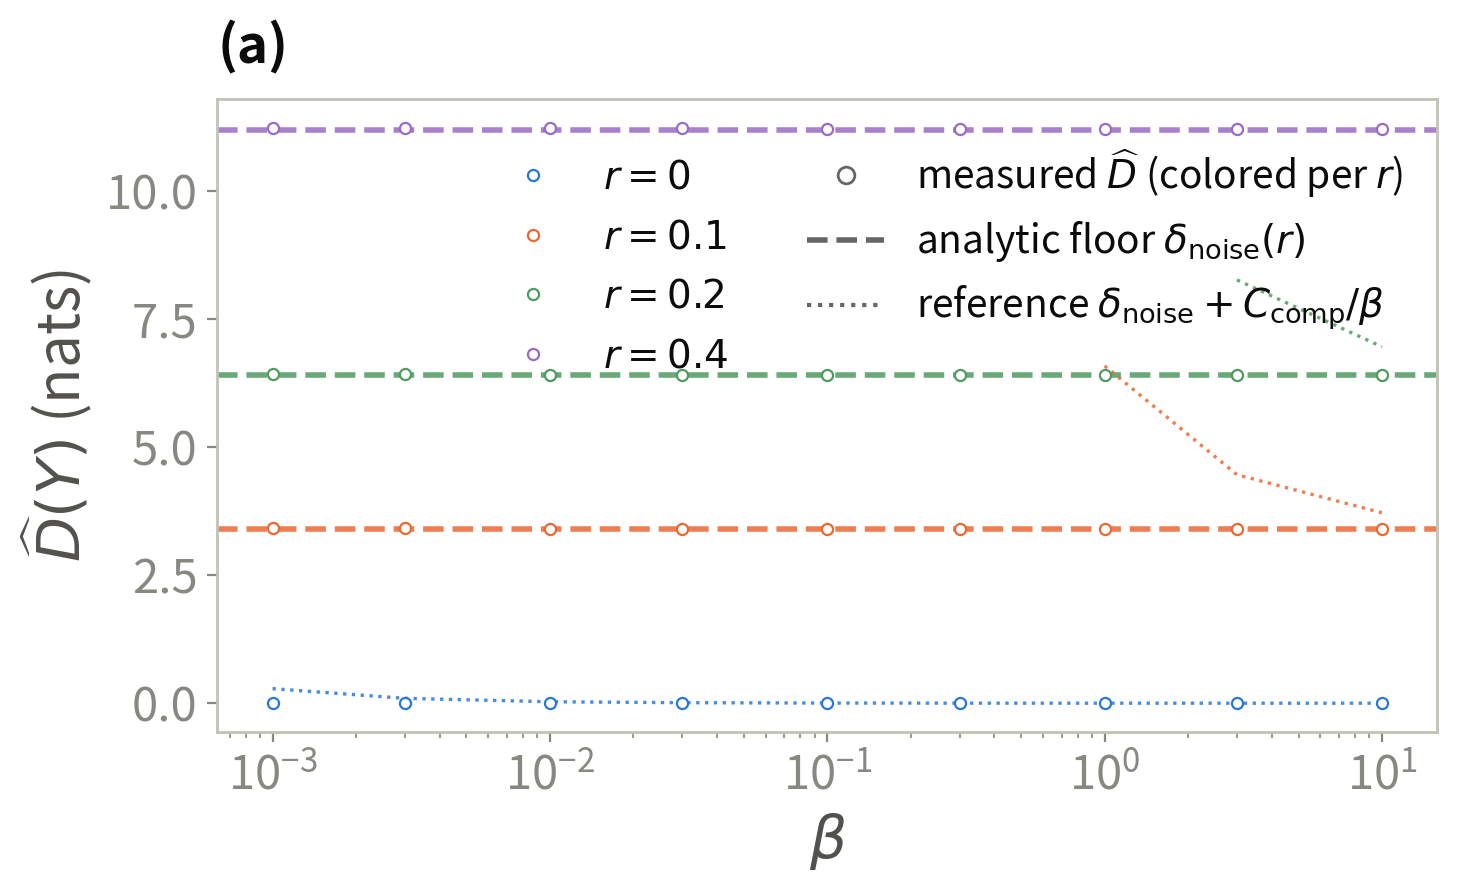
\includegraphics[width=0.32\linewidth]{figures/fig_noisy_appendix_i_varfixed.png}\hfill
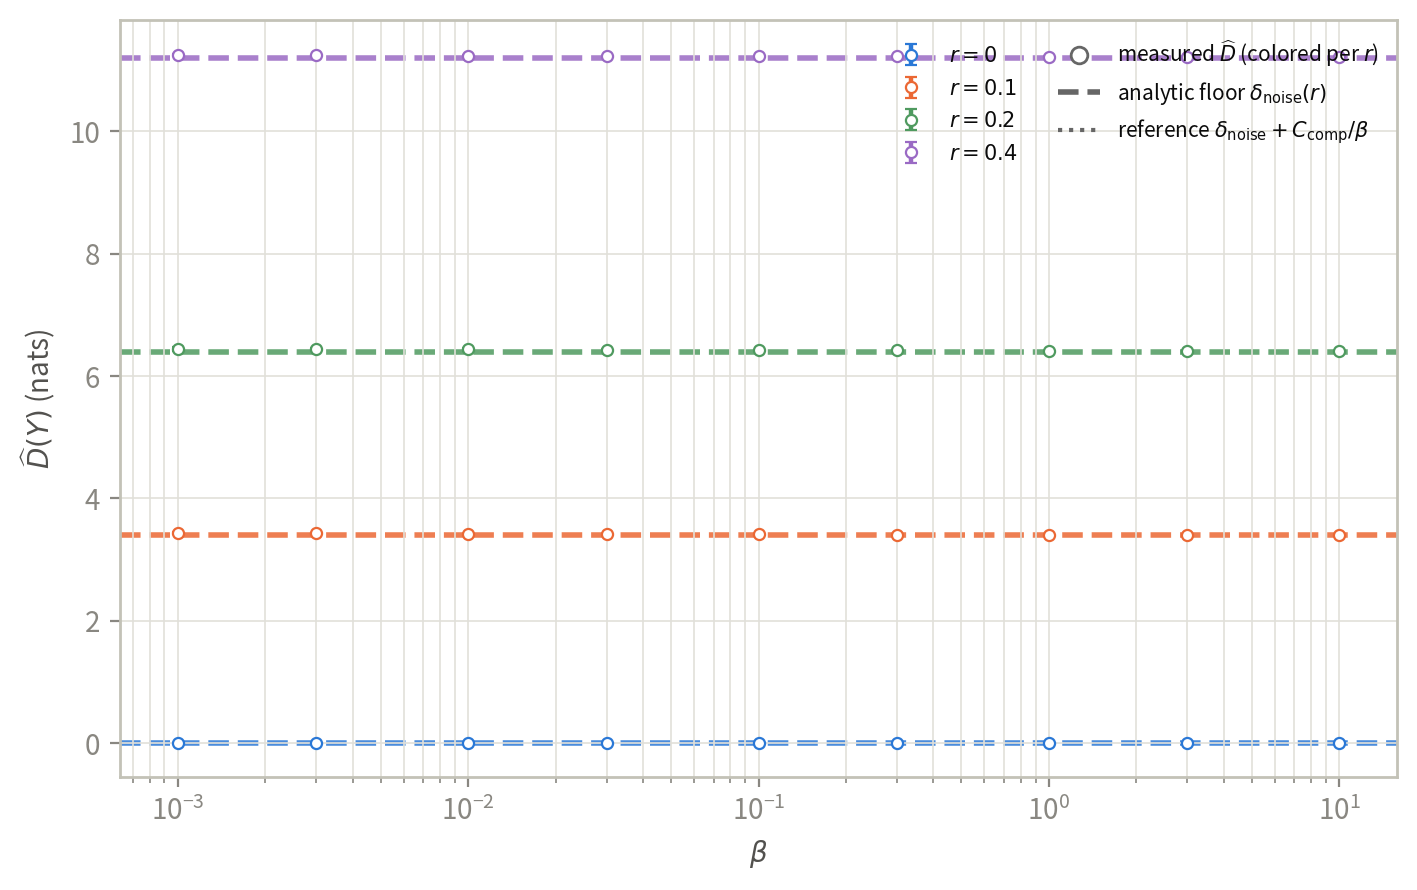
\includegraphics[width=0.32\linewidth]{figures/fig_noisy_appendix_ii_trainable.png}\hfill
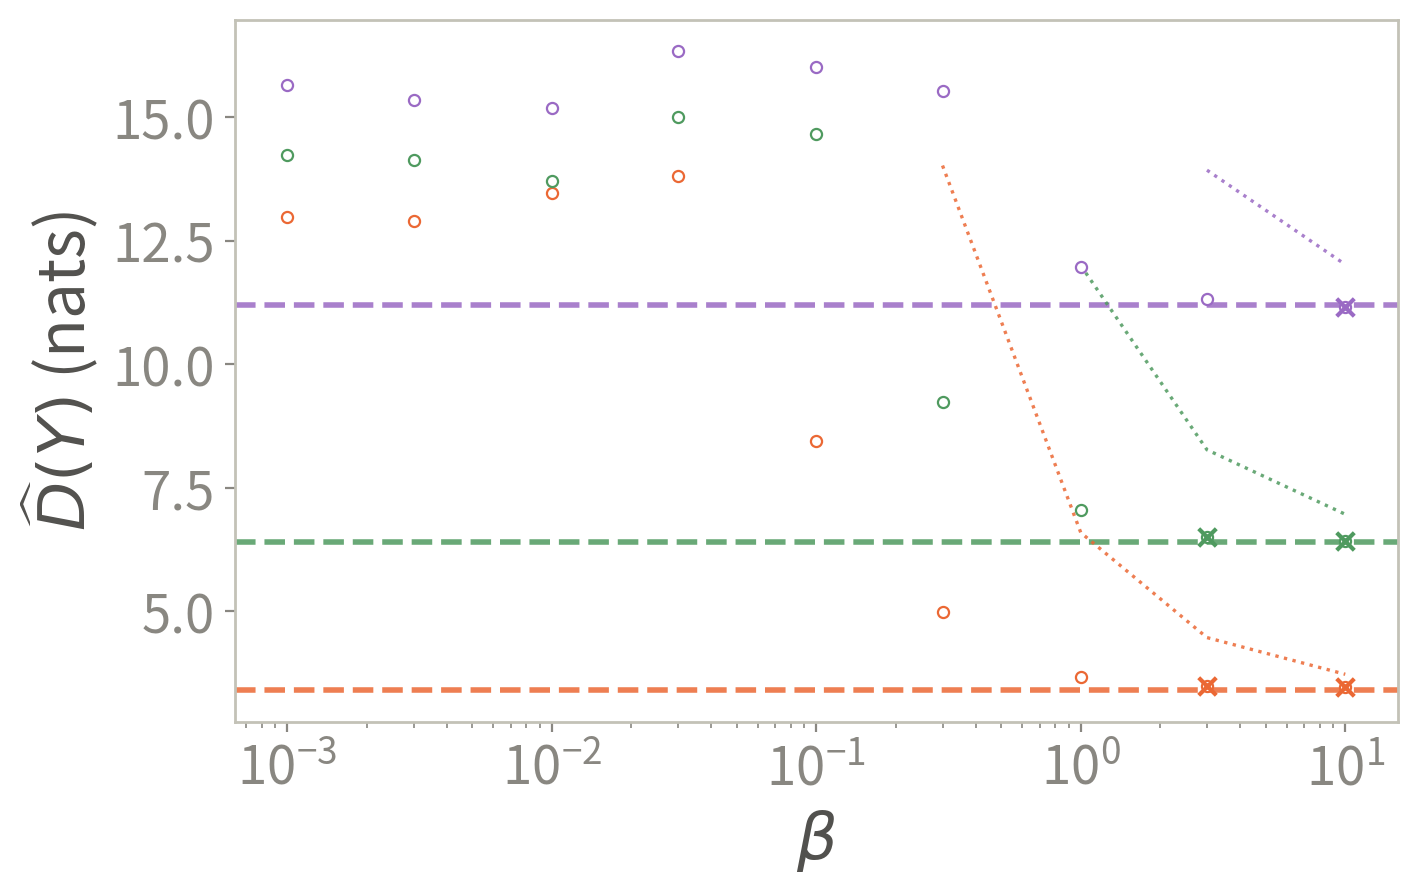
\includegraphics[width=0.32\linewidth]{figures/fig_noisy_appendix_iii_sampled.png}
\caption{Sensitivity analyses for the controlled label-ambiguity experiment.
(a) Posterior variance fixed to the prior variance. (b) Trainable polar
frame. (c) Labels sampled rather than integrated with their exact population weights;
failed comparator-gate configurations are marked. Dashed lines denote the analytic
population ambiguity floors. Points are means and error bars are standard deviations
over seeds.}
\label{fig:noisy-alignment-sensitivity}
\end{figure*}
\subsection{Alignment and separation: definitions and diagnostics}
\label{app:direct-mismatch}

This section collects the diagnostic panels deferred from
Section~\ref{sec:direct-mismatch}: the decoupling scatter, the separation-bound and
slack readings, and the regression diagnostics, together with the finite-bin
definitions. All statistics are first computed within each seed and then aggregated
across seeds; class or bin pairs are not treated as independent
replicates. The per-class Jensen check and the per-pair separation bound are
verified numerically on every scale, $\beta$, seed, and class (no violation exceeds
$10^{-6}$). Every checkpoint in both requested grids is present, and no collapse or
variance-explosion point is removed.

The deferred classification panels complete the picture
(Fig.~\ref{fig:direct-mismatch-deferred}). The decoupling scatter (a) shows MC-10
accuracy staying within $82$--$86\%$ while $\widehat D$ spans three orders of
magnitude: mechanism and task metric are decoupled. Panel (b) shows the raw bound
rising toward the declared $\sqrt2a$ exactly where the mismatch corrections shrink,
so the slack narrows where the bound is informative; CEB's mismatch is plotted
descriptively, without a bound or slack entries, since its reference has no declared
$\Delta$. The
slack percentiles (c) stay non-negative at every reported point: the bound is
consistent but conservative.

\begin{figure*}[t]
\centering
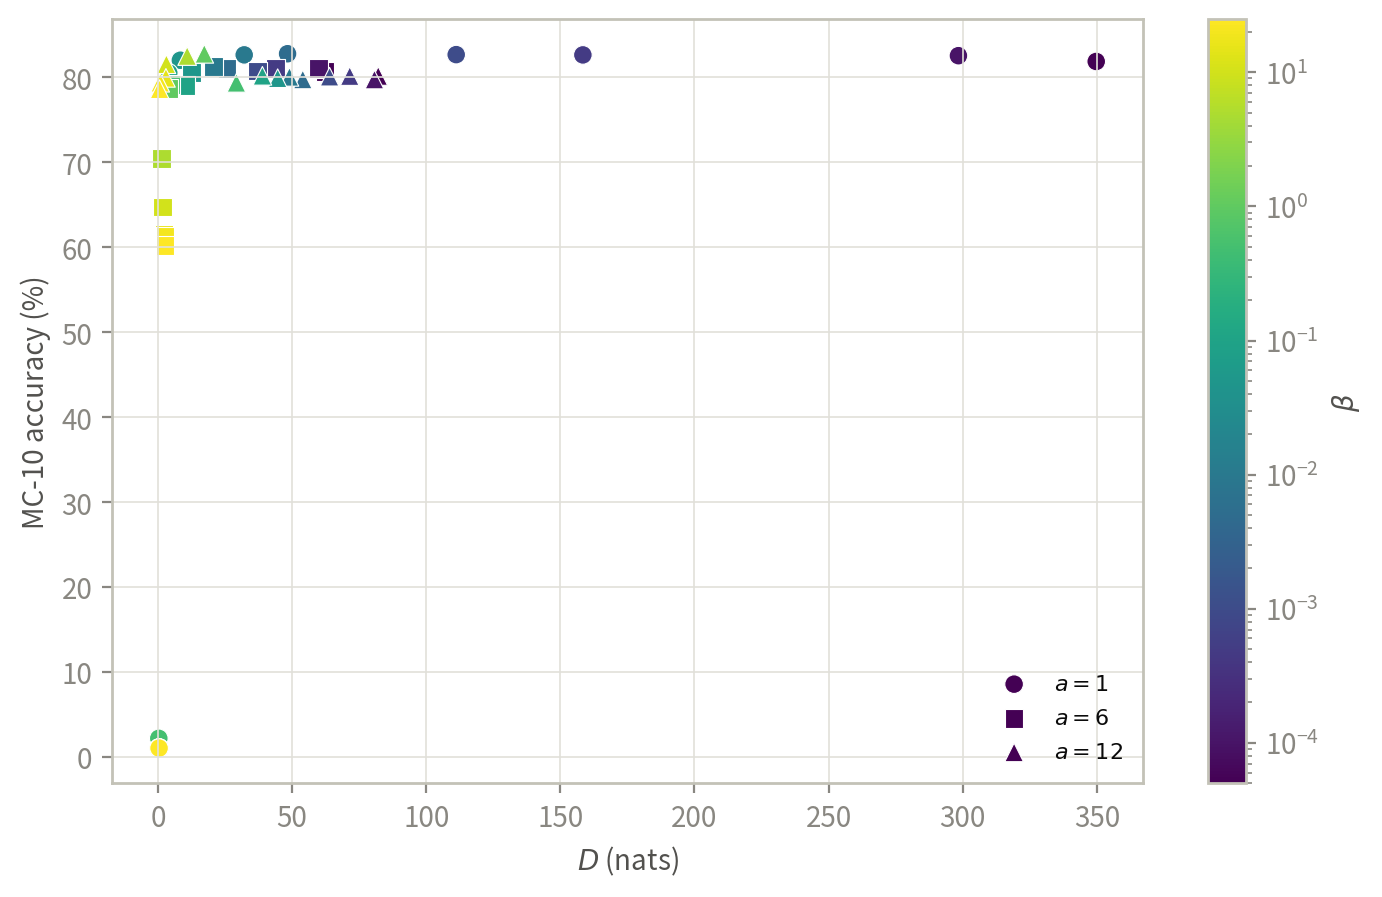
\includegraphics[width=0.24\linewidth]{figures/fig_mismatch_b_imagenet100_acc_vs_d.png}\hfill
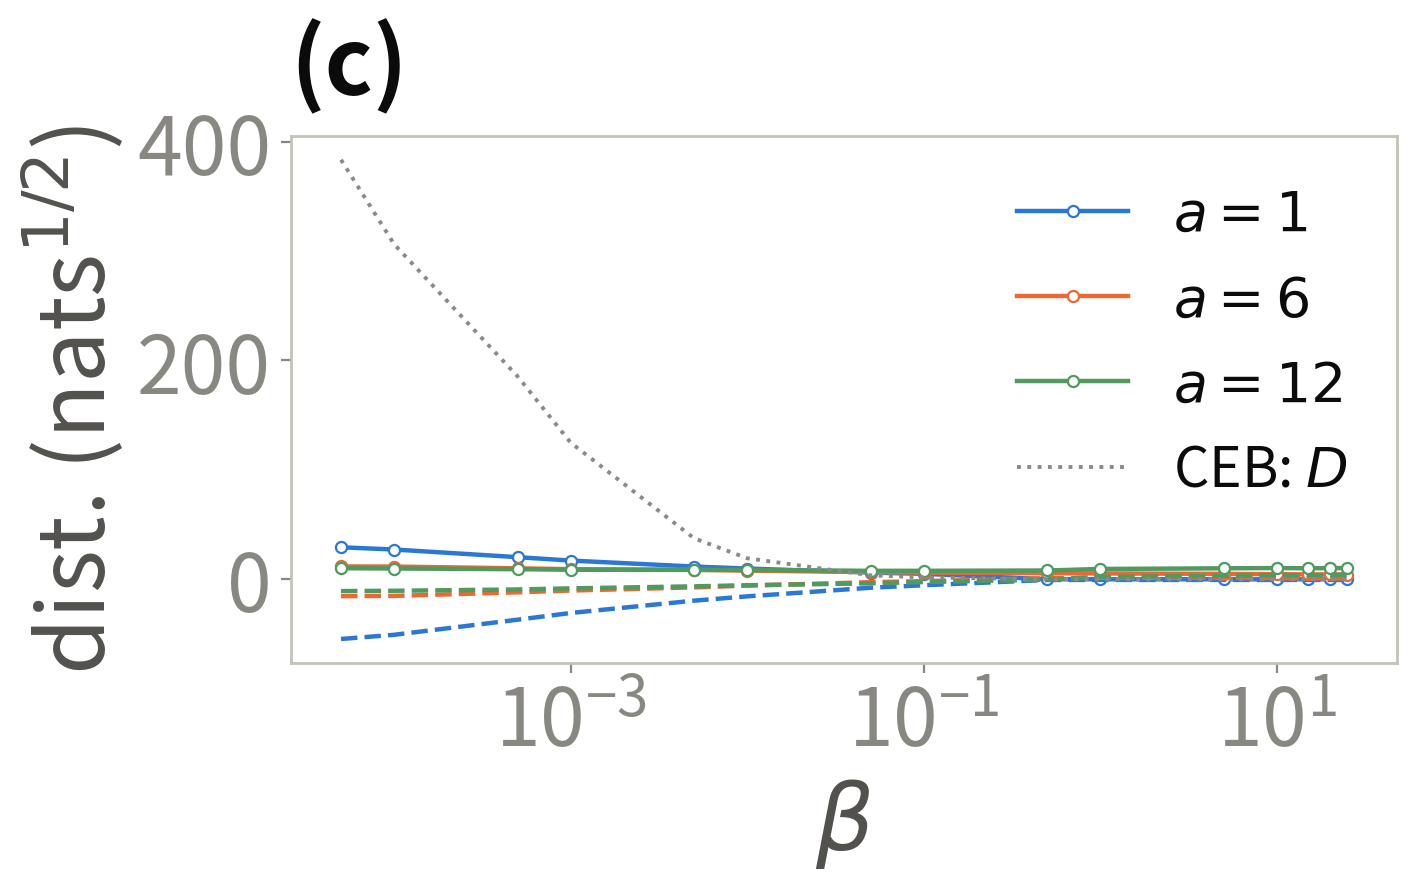
\includegraphics[width=0.24\linewidth]{figures/fig_mismatch_appendix_cls_i_separation_beta.png}\hfill
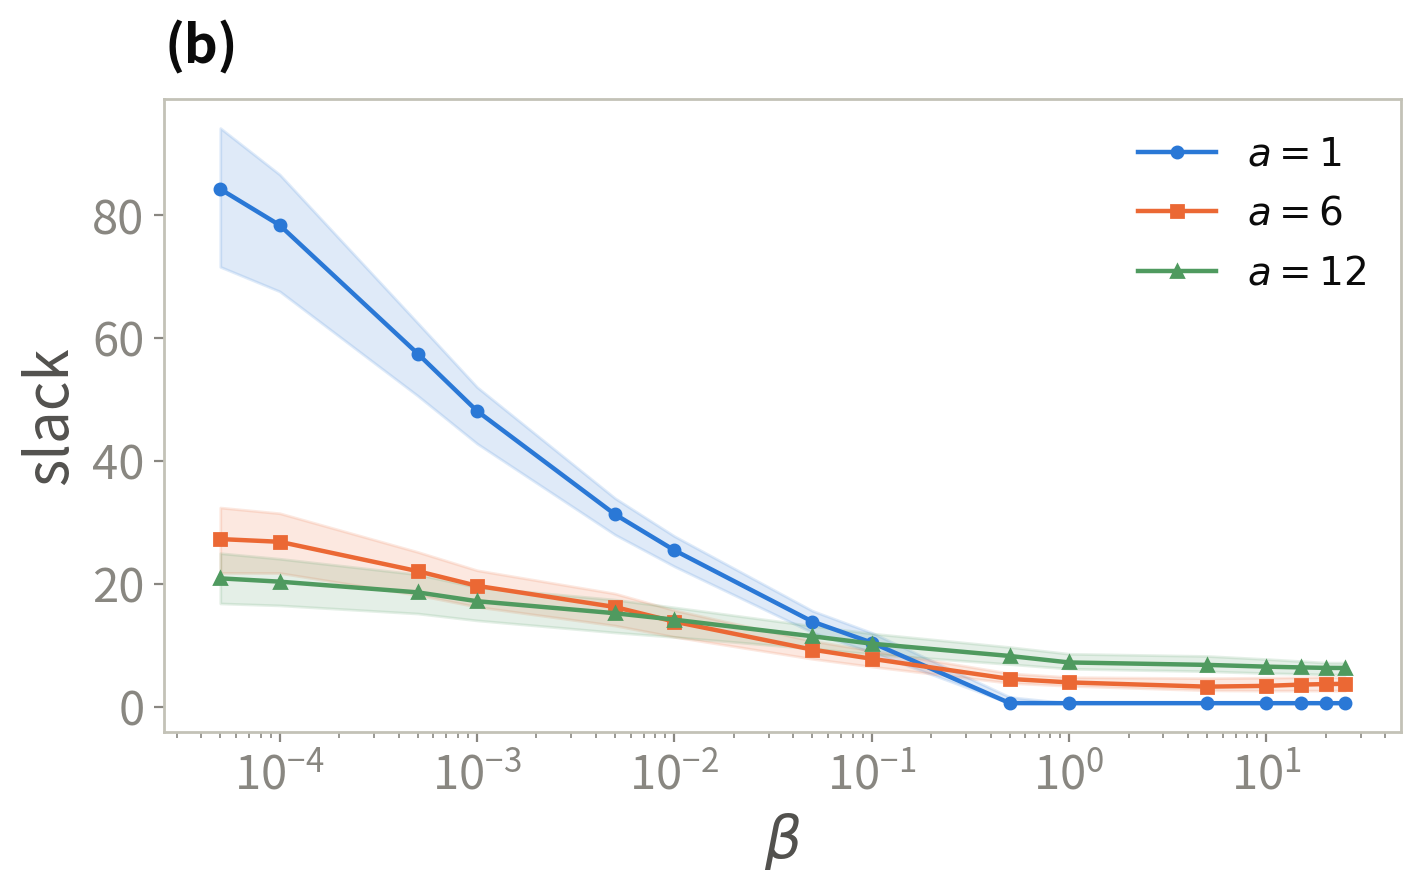
\includegraphics[width=0.24\linewidth]{figures/fig_mismatch_appendix_cls_iii_slack.png}\hfill
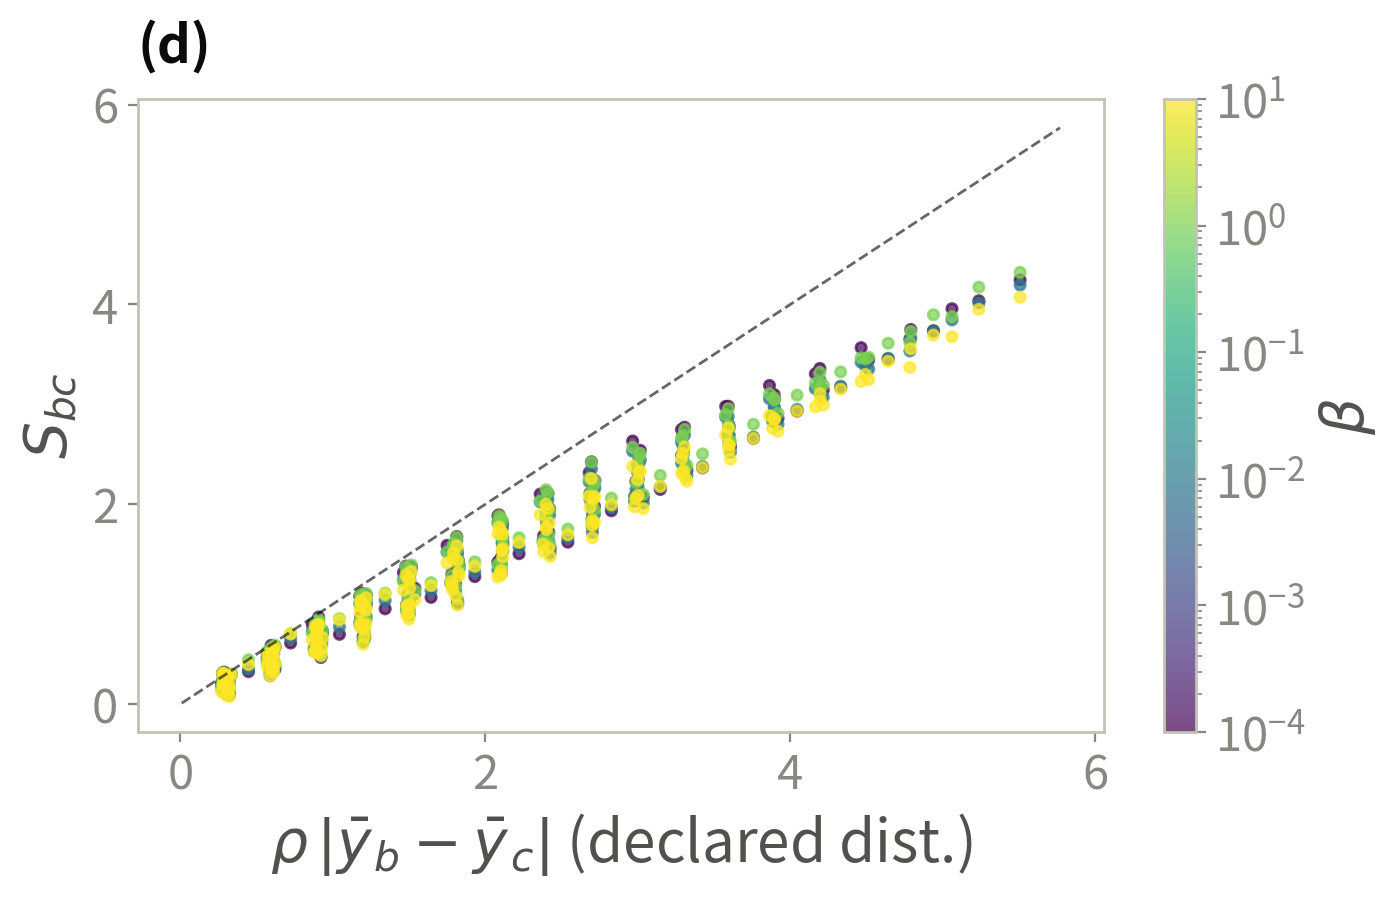
\includegraphics[width=0.24\linewidth]{figures/fig_mismatch_appendix_reg_binscatter.png}
\caption{Alignment and separation diagnostics deferred from the main text. (a) MC-10
accuracy against $\widehat D$ (color $=\beta$, marker $=a$). (b) Mean separation
(solid) and raw lower bound (dashed) against $\beta$; gray dotted: CEB,
descriptive. (c) Slack percentiles. (d) Cal.\ Housing bin-pair separation against
the declared prior distance at $\rho=6$ (color $=\beta$; identity line: exact
transfer).}
\label{fig:direct-mismatch-deferred}
\end{figure*}

\paragraph{Regression.} We partition the normalized test labels into $20$
equal-width bins and merge any bin containing fewer than $30$ examples. Let
$\bar y_b$ be the mean label of bin $B_b$, $\widehat{\bar\mu}_b$ its posterior center,
$\widehat D_b$ its average sample-to-own-anchor mismatch, and
$h_b:=\operatorname{diam}(B_b)$. The finite-bin lower bound is
\begin{equation}
\widehat{\mathrm{LB}}_{bc}
=\rho|\bar y_b-\bar y_c|
-\sqrt{2\tau^2\widehat D_b}
-\sqrt{2\tau^2\widehat D_c}
-\rho(h_b+h_c),
\label{eq:empirical-regression-separation-bound}
\end{equation}
where the last term is the quantization correction of
Remark~\ref{rem:pgib-binning}. On Housing with $\rho=6$, mismatch falls from
$0.264$ to $0.026$, the axial slope remains $0.73$--$0.77$, and the mismatch is
almost entirely axial (about $0.2$ against $0.004$ off-axis), while $R^2$ changes
only from $0.786$ to $0.767$ over the sweep: a tenfold mismatch reduction need not
imply a comparable task-metric gain. Figure~\ref{fig:direct-mismatch-deferred}d
plots the actual bin-center distances against the declared isometric distances at
$\rho=6$: the cloud hugs a line of slope $0.73$--$0.77$ below the identity line at
all four $\beta$ values, so the posterior follows the declared metric structure at
about three quarters of its scale, and the scale-transfer ratio is essentially
$\beta$-invariant. After the quantization correction, $43\%$ of bin pairs retain a
positive bound. Figure~\ref{fig:direct-mismatch-housing} shows the two regression
sweep panels: the mismatch--$\beta$ curves with their axial/off-axis decomposition
(the dotted off-axis contribution stays below $0.01$ nats, so the posterior lies
essentially on the declared axis), and the $R^2$-against-$\widehat D$ scatter whose
band stays within $0.75$--$0.79$ while $\widehat D$ spans orders of magnitude.

\begin{figure*}[t]
\centering
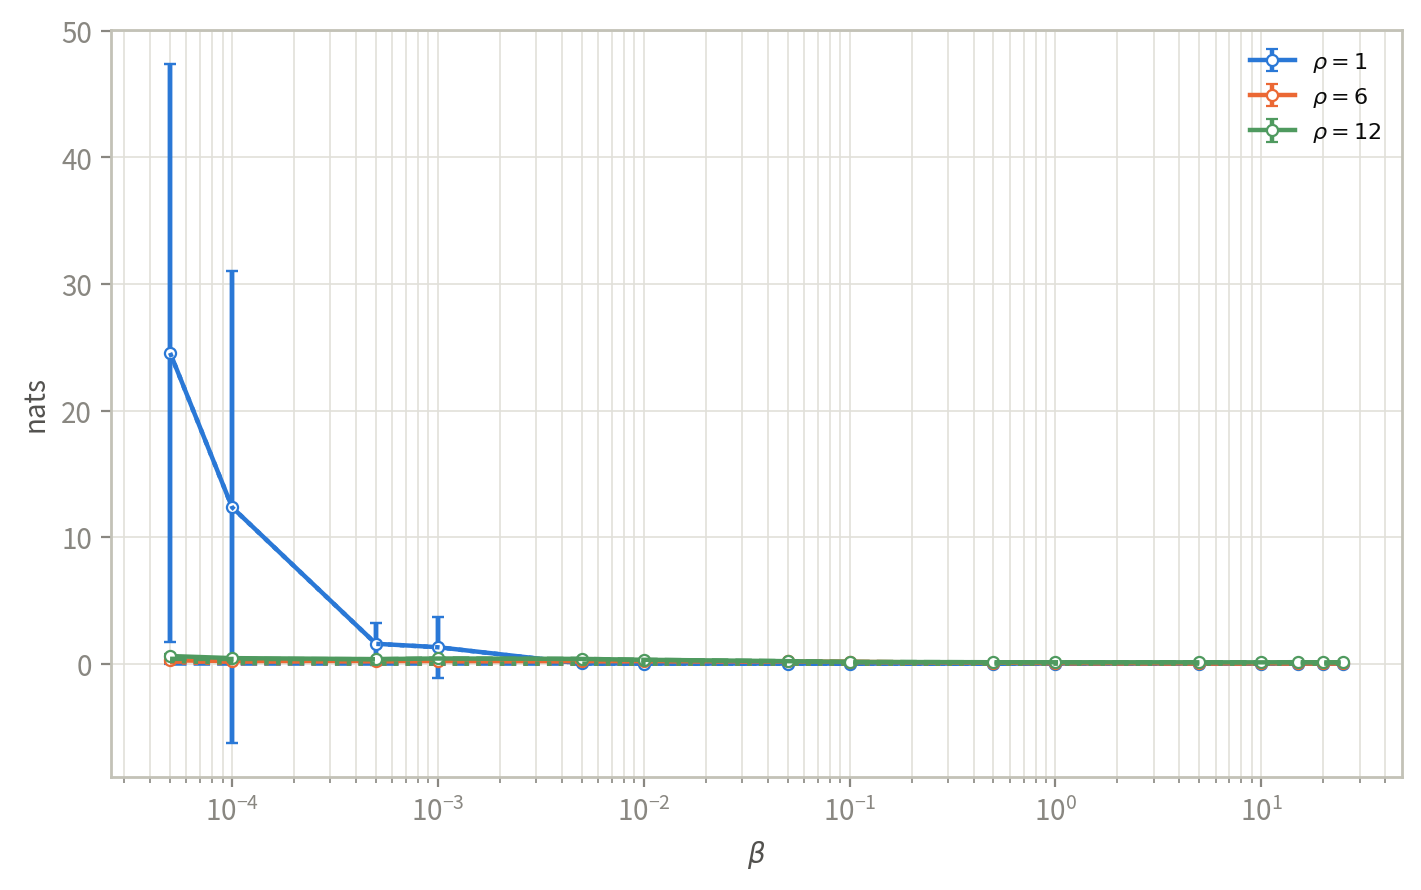
\includegraphics[width=0.48\linewidth]{figures/fig_mismatch_c_housing_d_beta.png}\hfill
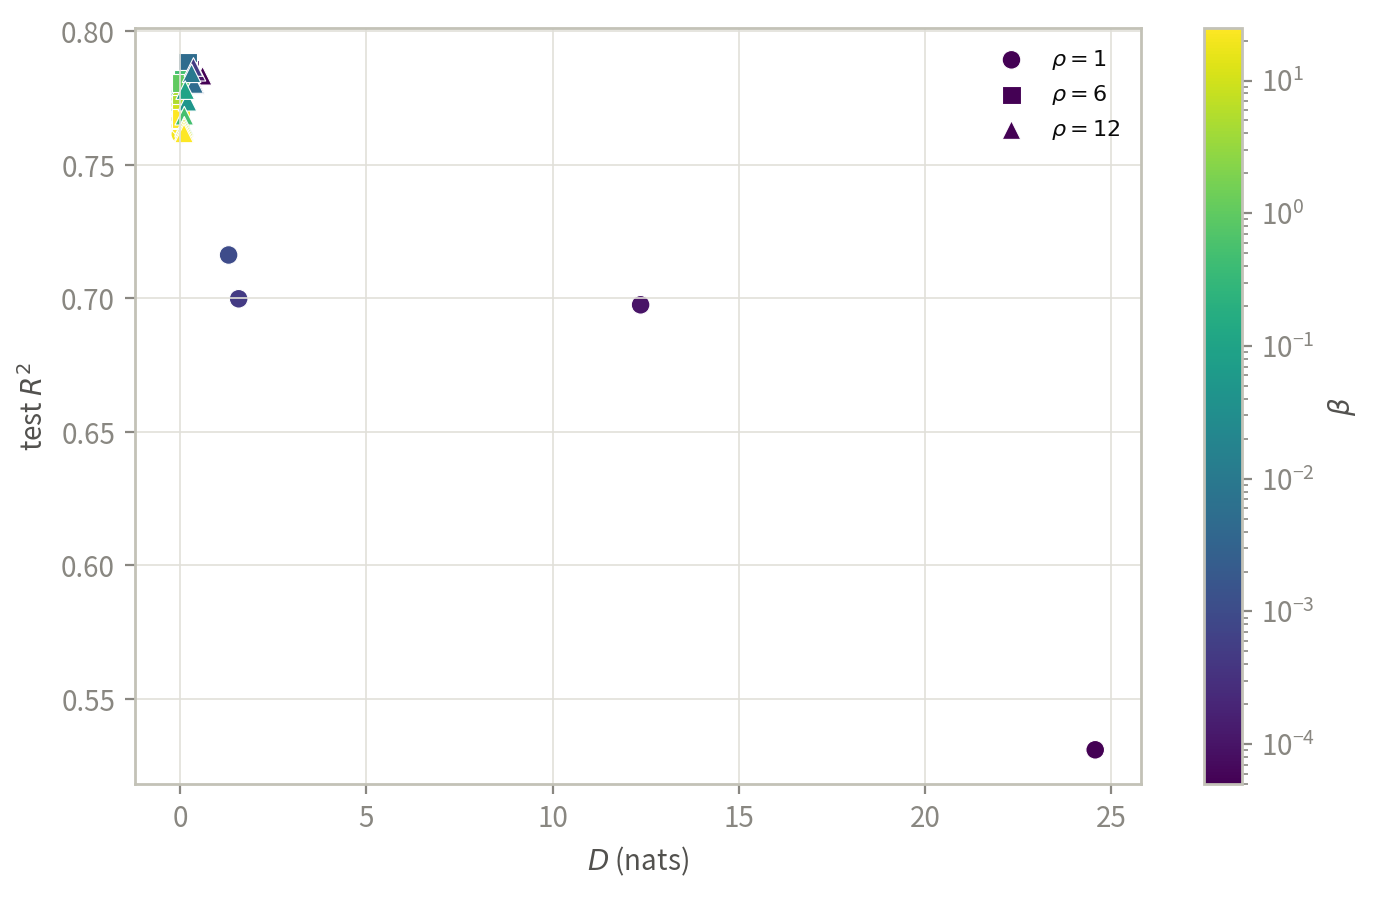
\includegraphics[width=0.48\linewidth]{figures/fig_mismatch_d_housing_r2_vs_d.png}
\caption{Cal.\ Housing mismatch sweep panels (deferred from the main text). (a)
Anchor mismatch $\widehat D$ against $\beta$, by isometric scale $\rho$, decomposed
into axial and off-axis contributions. (b) Test $R^2$ against $\widehat D$; color
denotes $\beta$ and marker shape $\rho$.}
\label{fig:direct-mismatch-housing}
\end{figure*}

\paragraph{Normalization and variance extremes.} The empirical mismatch normalizes
by the declared prior variance $\tau^2=1$, whereas the
exact Gaussian KL uses every sample's and coordinate's own posterior variance
$\sigma^2_\phi(x)$. They therefore need not coincide: averaged over the ImageNet-100
grid, $\widehat D=41.2$, the KL mean term is $46.5$, and the KL variance term is
$51.4$. On Housing, a small number of weak-compression, large-$\rho$ posterior
variance explosions raise the across-grid mean KL variance term to $2.8\times10^6$;
these checkpoints remain in all plots. The unnormalized axial/off-axis components and
total KL are therefore reported alongside $\widehat D$.
\subsection{Adversarial robustness details}
\label{app:robustness}
Targeted PGD uses 20 steps, EOT-10 gradients, 10-sample MC predictions, and budgets
$\varepsilon_\infty=0.3$ and $\varepsilon_2=6$. Curves are shown only when clean
stochastic accuracy exceeds $90\%$. At maximum compression, OPB $(a=6,12)$ reaches
$31.1\%/30.5\%$ targeted success under $L_\infty$, while transfer attacks from CEB
to OPB reach at most $2.0\%$/$3.4\%$ under $L_\infty/L_2$, far below OPB's white-box
attack. The transfer result is a gradient-masking check rather than a causal geometry
test.

\begin{figure*}[t]
\centering
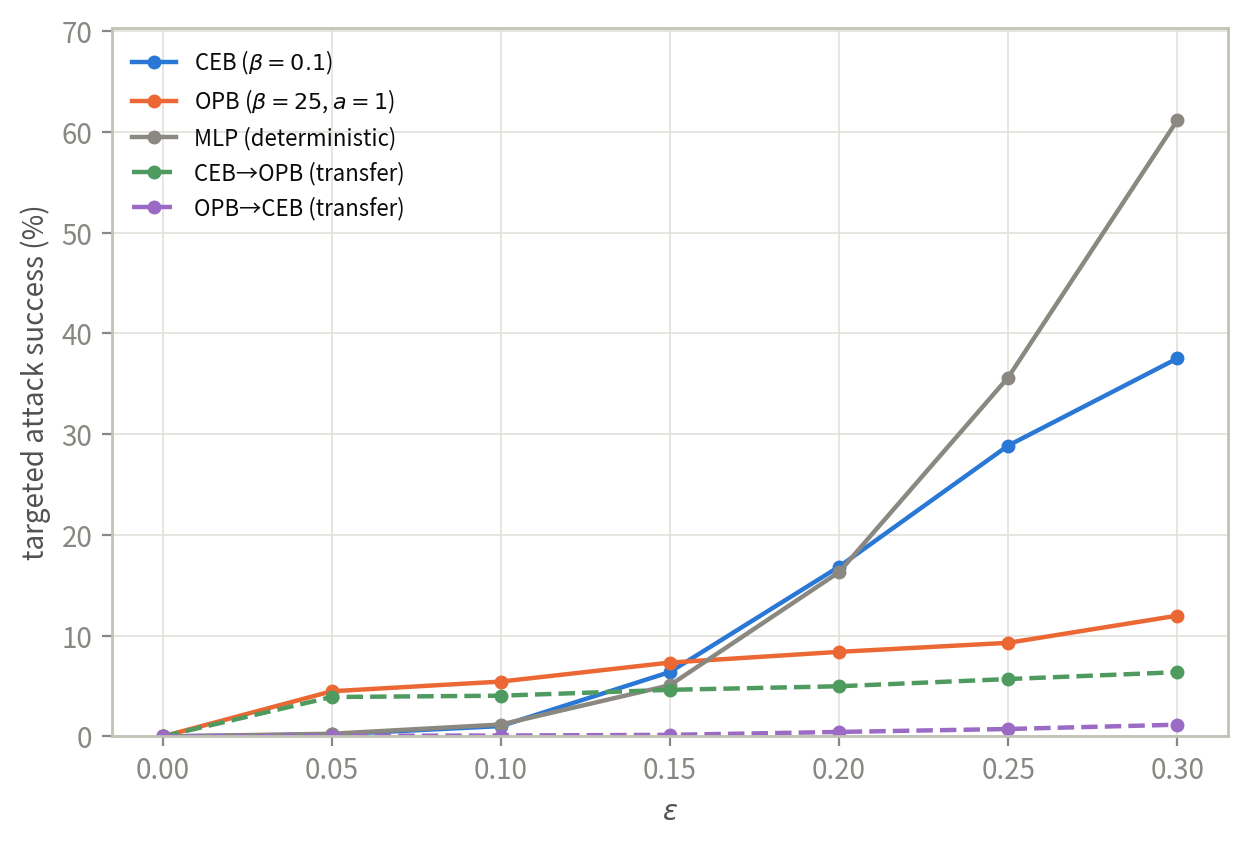
\includegraphics[width=0.48\linewidth]{figures/fig_adv_transfer_linf_mnist.png}\hfill
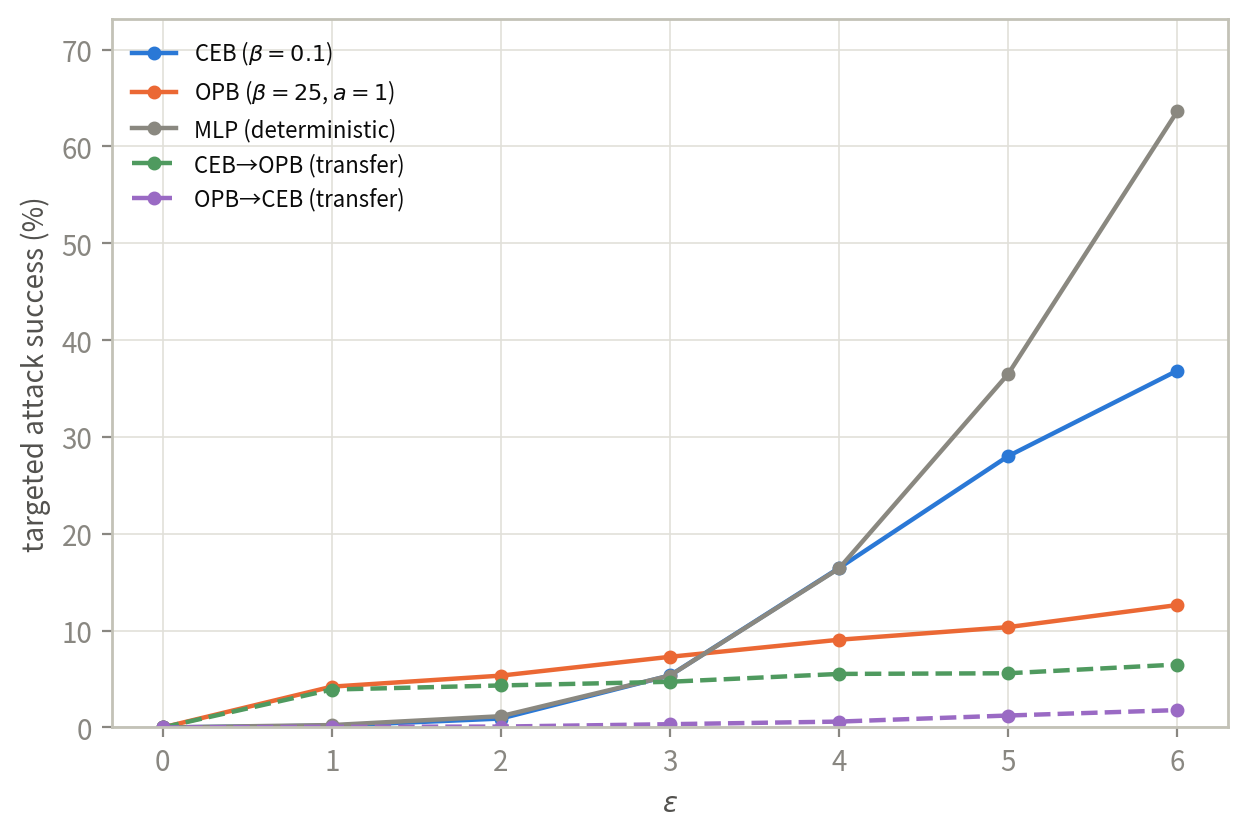
\includegraphics[width=0.48\linewidth]{figures/fig_adv_transfer_l2_mnist.png}
\caption{Transfer PGD curves on MNIST (gradient-masking check). Targeted adversaries
are generated on one model and evaluated on another; CEB-to-OPB transfer remains far
below OPB's own white-box attack. The targeted white-box curves are in the main text.}
\label{fig:adv-transfer}
\end{figure*}
\subsection{Factor-wise ablations}
\label{app:ablation}
The factor-wise ablation ladder switches geometry, anchor scale, readout, and the IB
term separately; each variant is evaluated at its best validation-selected
configuration (Table~\ref{tab:ablation}). The complete means are reported in
Table~\ref{tab:ablation}. The paired bootstrap intervals are in the main text
(Table~\ref{tab:ablation-ci}) for the classification contrasts and in
Table~\ref{tab:ablation-ci-epb} for the regression mirrors; all paired differences
use the shared seeds at each variant's best validation-selected configuration,
and the intervals are $95\%$ bootstrap percentile CIs with $B=10{,}000$ and a fixed
seed. The factor ranking and
the sign-flip and negative-result patterns are read in the main text
(Section~\ref{sec:ablation}).

\emph{NCM-learn} removes the bottleneck entirely: the encoder output is used
deterministically ($z=\mu_\phi(x)$, no posterior and no KL) and classified by an
energy readout on trainable prototypes. \emph{NCM-ortho} is the same, except that
the prototypes are fixed to the orthogonal frame $a\,e_k$ (fixed geometry, still no
IB). \emph{CEB-energy} and \emph{CEB-tied} keep CEB's trainable free reference and
KL but replace its free head by the energy readout (resp.\ the tied projection).
\emph{OPB-FS} and \emph{EPB-FS} keep the orthogonal frame and the energy (resp.\
tied) readout but make the anchor radius learnable, so only the fixed scale is
switched off. \emph{GPB-L} is GPB's free-head counterpart on the classification
settings (identical orthogonal-frame prior, free linear head), and \emph{EPB-L}
and \emph{EPB} are the regression counterparts of GPB-L and GPB on Housing,
keeping the isometric-axis prior with a free head (resp.\ the tied projection).
\emph{OPB-RV} freezes all trainable prior parameters on the classification
settings, and \emph{EPB-RV} freezes all trainable prior parameters on the
regression settings.

\begin{table}[t]
\centering
\small
\caption{Attribution ablation: best-configuration test metrics (mean $\pm$ std
over seeds). Configurations are selected by the mean validation metric
(accuracy on MNIST and ImageNet-100), applied identically to
every variant, so all comparisons remain paired by seed and the test split is
never touched by selection. One OPB-FS configuration (ImageNet-100,
$\beta = 10^{-4}$, $a = 1$) diverged during training (free scales grow without
penalty at negligible $\beta$) and is excluded.}
\label{tab:ablation}
\begin{tabular}{l c c}
\hline
variant & MNIST (Acc \%) & ImageNet-100 (Acc \%) \\
\hline
Base & $98.33 \pm 0.12$ & $83.12 \pm 0.14$ \\
NCM-learn & $98.17 \pm 0.17$ & $82.17 \pm 0.36$ \\
NCM-ortho & $98.11 \pm 0.12$ & $82.33 \pm 0.60$ \\
CEB & $98.43 \pm 0.08$ & $82.78 \pm 0.22$ \\
CEB-energy & $98.22 \pm 0.10$ & $81.59 \pm 0.21$ \\
GPB-L & $98.43 \pm 0.07$ & $83.40 \pm 0.67$ \\
GPB & $98.44 \pm 0.08$ & $84.22 \pm 0.15$ \\
OPB-RV & $98.34 \pm 0.04$ & $83.38 \pm 0.52$ \\
OPB-FS & $98.54 \pm 0.03$ & $84.26 \pm 0.18$ \\
\hline
\end{tabular}
\end{table}


\begin{table}[t]
\centering
\tiny
\caption{Regression mirrors of the factor-wise paired differences ($R^2$ on
Housing; $95\%$ bootstrap percentile CIs; positive values favor the first
term).}
\label{tab:ablation-ci-epb}
\begin{tabular}{l l c}
\hline
factor & comparison & Housing \\
\hline
readout (EPB) & EPB $-$ EPB-L & $-0.00$ [$_{-0.01}$, $_{-0.00}$] \\
geometry (EPB) & EPB-FS $-$ CEB-tied & $+0.01$ [$_{-0.00}$, $_{0.01}$] \\
fixed scale (EPB) & EPB $-$ EPB-FS & $+0.00$ [$_{-0.01}$, $_{0.01}$] \\
frame trainability (EPB) & EPB $-$ EPB-RV & $-0.00$ [$_{-0.00}$, $_{0.00}$] \\
\hline
\end{tabular}
\end{table}

\emph{Reading the regression mirrors.} The frame-trainability contrast is a
null on Housing (Table~\ref{tab:ablation-ci-epb}): freezing all trainable prior
parameters costs nothing, so the trainable rotation carries no benefit in
regression, unlike the classification settings where it adds $+0.83$ on
ImageNet-100 (Table~\ref{tab:ablation-ci}).
\subsection{Regression compression curves}
\label{app:compression}
The main text shows the classification compression sweep. This companion figure gives
the complete California Housing regression sweep under the same $\beta$ grid, including
the weak-compression variance explosion and the strong-compression EPB plateau. The
curves are diagnostics of achieved KL and task performance, not tests of the alignment
rate.

\begin{figure*}[t]
\centering
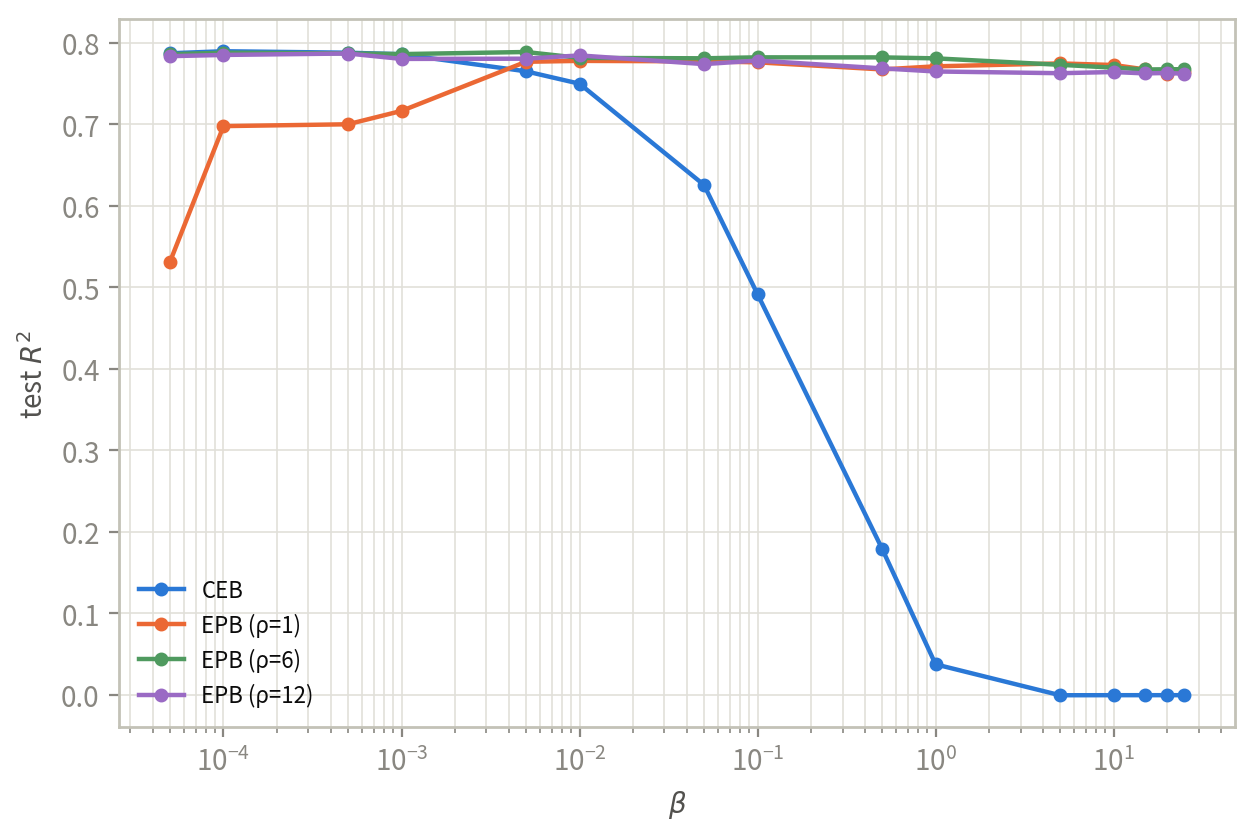
\includegraphics[width=0.48\linewidth]{figures/fig_beta_acc_housing.png}\hfill
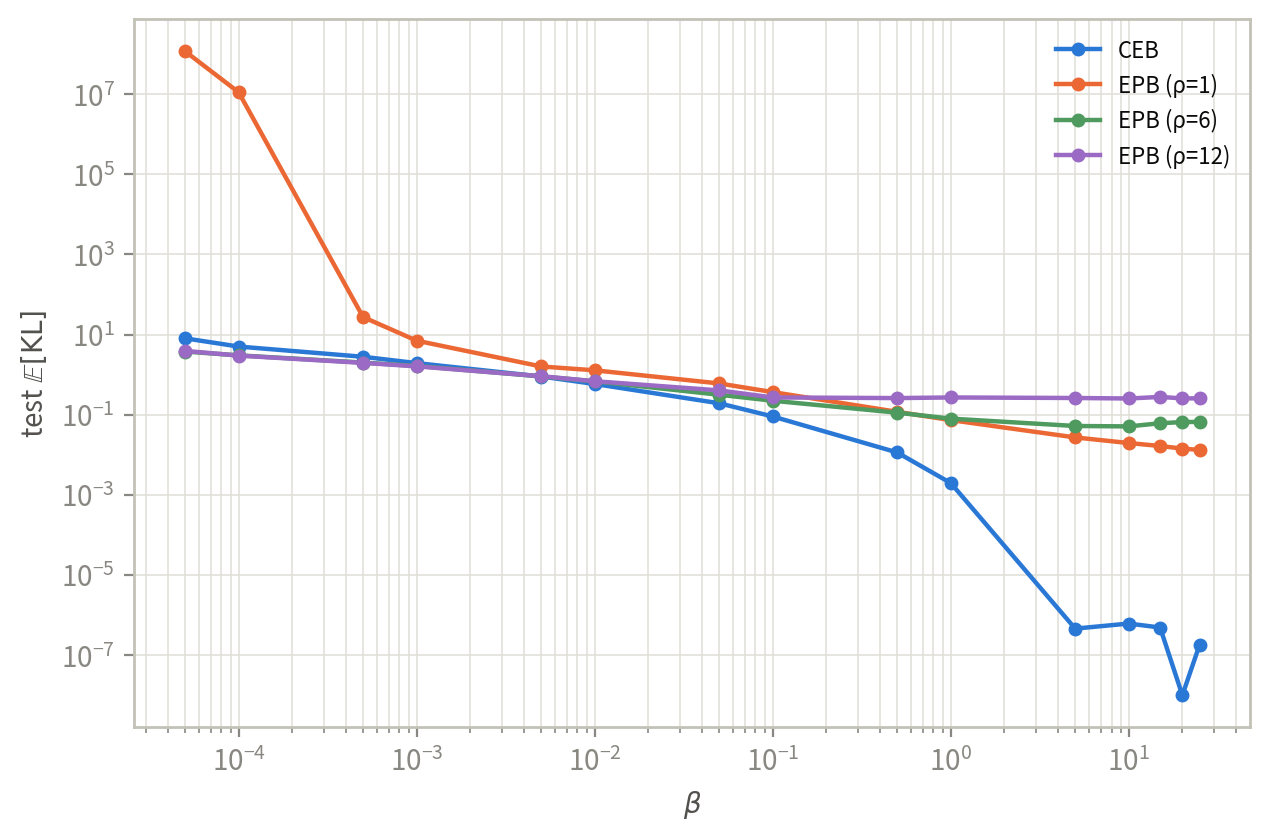
\includegraphics[width=0.48\linewidth]{figures/fig_beta_kl_housing.png}
\caption{California Housing compression sweep (MLP). Left: test $R^2$; right:
realized conditional KL over $\beta$. EPB maintains a task plateau through strong
compression, while the $\rho=1$ weak-compression points exhibit a large variance term.}
\label{fig:compression-housing}
\end{figure*}
\subsection{Anchor-scale sensitivity}
\label{app:scale-sensitivity}
The main comparison selects the prior scale on the five-value grid
$\{1,3,6,9,12\}$ (Sec.~\ref{sec:setup}); Fig.~\ref{fig:scale-sensitivity} reads the full
five-point scale grid at weak, medium, and strong compression on the two
representative settings, complementing the $\beta$-axis
sweeps of Sec.~\ref{sec:sweep} with the scale-axis view.

\begin{figure*}[t]
\centering
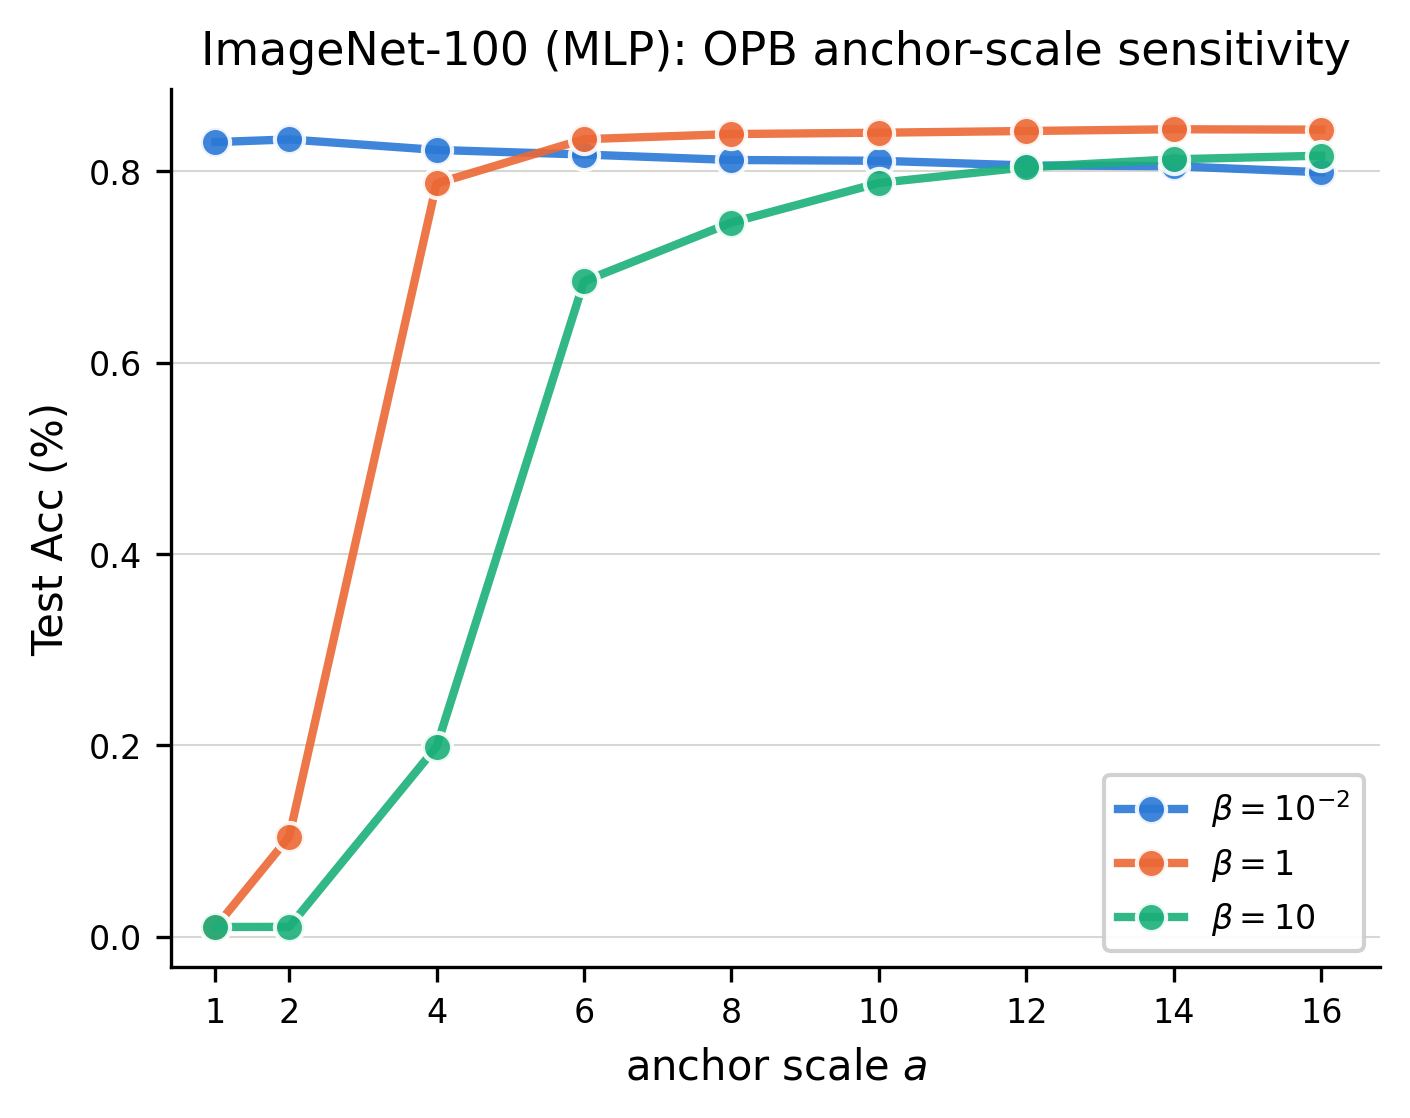
\includegraphics[width=0.49\linewidth]{figures/fig_anchor_sensitivity_imagenet100_mlp.png}\hfill
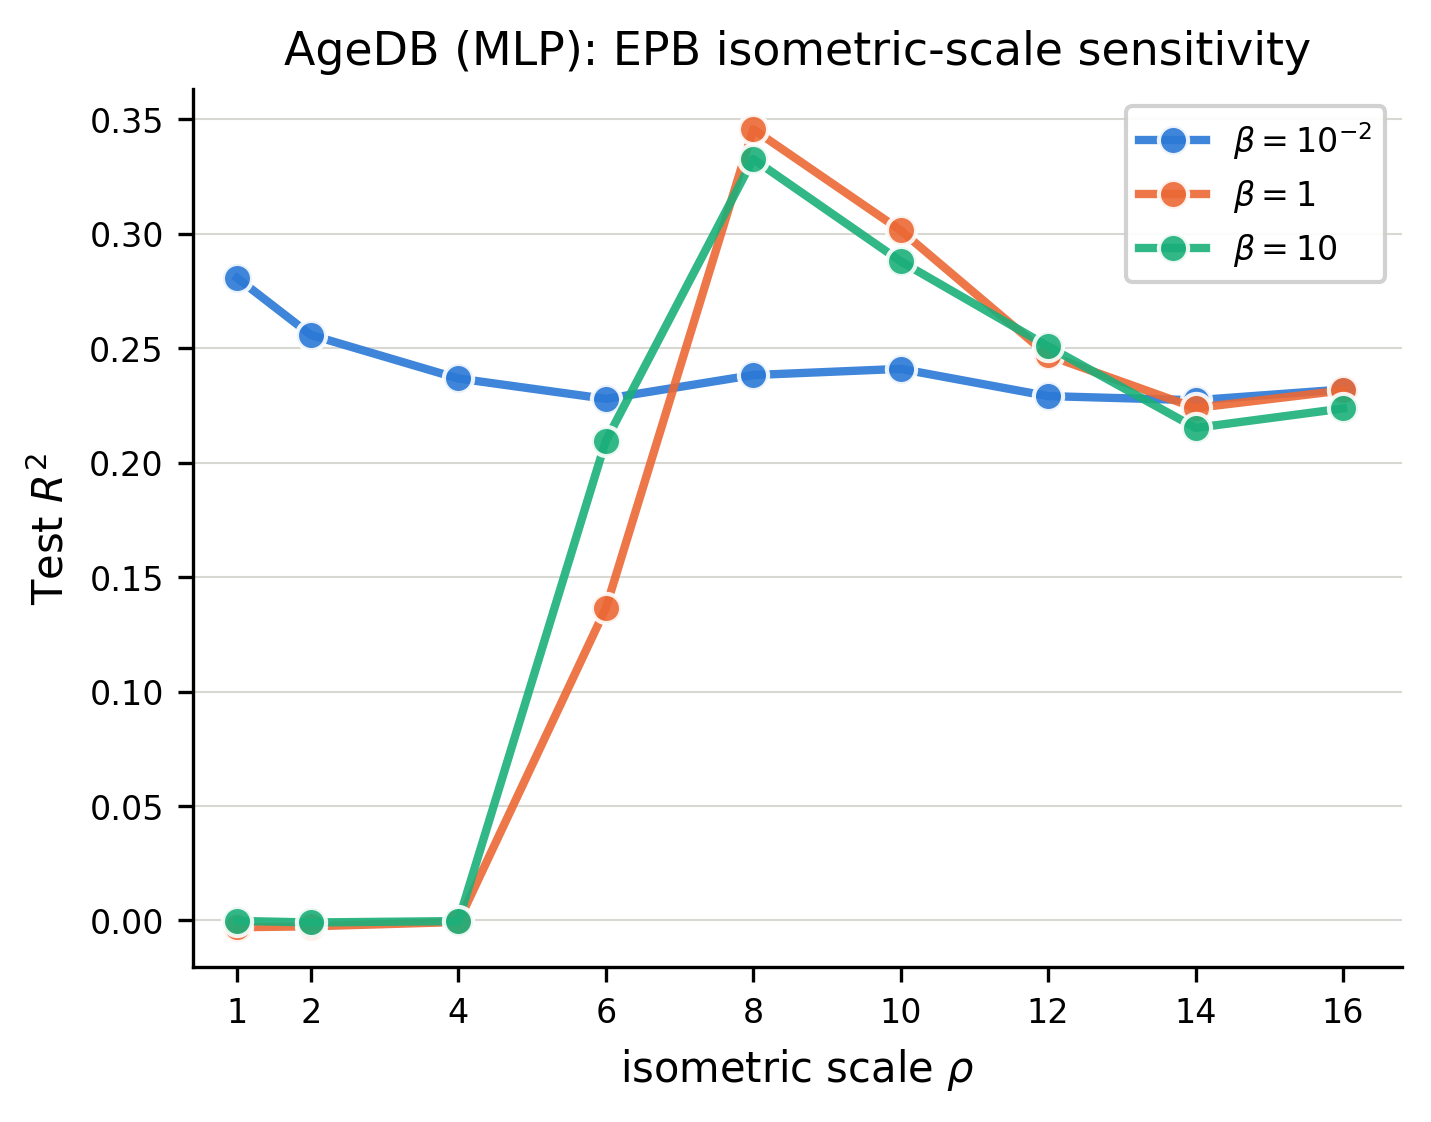
\includegraphics[width=0.49\linewidth]{figures/fig_anchor_sensitivity_agedb_mlp.png}
\caption{Anchor-scale sensitivity: (a) ImageNet-100 (MLP) OPB test accuracy
against the anchor scale $a$; (b) AgeDB (MLP) EPB test $R^2$ against the
isometric scale $\rho$; $\beta\in\{10^{-2},1,10\}$ (weak/medium/strong
compression).}
\label{fig:scale-sensitivity}
\end{figure*}

On both settings the scale matters only once compression bites: the
weak-compression curves are flat (within $3.4$ points on ImageNet-100),
and at $\beta\ge1$ scales below $4$ collapse (to chance accuracy on
ImageNet-100, to zero $R^2$ on AgeDB) while every scale above $6$ stays
on a plateau; the operating point is therefore sensitive to the scale
only through this collapse boundary, and the selected scale
lies inside the retained band.
\subsection{Information-plane estimates}
\label{app:info-plane}
Estimator protocol.\ $I(X;Z)$ is estimated by the InfoNCE lower bound
\citep{oord2018representation} ($\log N_{\rm neg}-\mathcal{L}_{\mathrm{NCE}}$, $N_{\rm neg}=4096$; one
critic per run, trained on the training split, the bound read off the test split with
$z\sim q(z|x)$). $I(Y;Z)$ is read on the same sampled posterior: $H(Y)-\mathrm{CE}$
with the cross-entropy averaged over $M=20$ draws $z\sim q(z|x)$ per test point
(still a lower bound, as $\mathrm{CE}\ge H(Y|Z)$). The residual $I(X;Z|Y)$ is
estimated directly rather than as a difference: every $q(z|x)$ is a known Gaussian,
so the class-conditional mixture
$q(z|y)=\frac{1}{N_y}\sum_{j:y_j=y}q(z|x_j)$ over the test samples is evaluated
exactly by logsumexp, and
$I(X;Z|Y)=\mathbb{E}_{x,y}\,\mathrm{KL}(q(z|x)\,\|\,q(z|y))$ is read by Monte
Carlo---an exact estimate up to $z$-sampling noise and the finite per-class test
sample, not a difference of bounds. The certificate-plane axis is drawn linear
because the collapsed CEB trajectory lands on zero. The MNIST panels appear in
Fig.~\ref{fig:compression-main}(c,d) of the main text.

Matched-compression performance.
Table~\ref{tab:info-plane-matched} pairs each CEB point with the OPB configuration of
nearest estimated $I(X;Z)$. At $\approx2.0$ nat, CEB ($\beta=0.5$) retains $86.0\%$
while OPB ($a=1$, $\beta=0.5$) retains $97.8\%$; at $\approx2.5$ nat ($\beta=0.1$) the
two tie ($98.2\%$ vs.\ $98.1\%$). The directly estimated residual is comparable or
slightly larger for OPB at both points ($0.41$ vs.\ $0.47$ nat at $\beta=0.1$;
$0.20$ vs.\ $0.21$ nat at $\beta=0.5$), so OPB's task plateau is not bought by extra
residual compression. These are paired empirical comparisons at two estimated
compression levels, not a causal attribution to geometry.

\begin{table}[t]
\centering\small
\setlength{\tabcolsep}{4pt}
\caption{Matched-compression information-plane comparison (means; standard deviations
are in the stored evaluation report). The OPB configuration is the one whose
estimated $I(X;Z)$ is nearest to the CEB point.}
\label{tab:info-plane-matched}
\begin{tabular}{l c c c l c c c}
\hline
& \multicolumn{3}{c}{CEB} & \multicolumn{4}{c}{OPB}\\
\cline{2-4}\cline{5-8}
Setting & $I(X;Z)$ & $I(X;Z|Y)$ & Acc. & config. & $I(X;Z)$ & $I(X;Z|Y)$ & Acc.\\
\hline
MNIST, $\beta=0.1$ & $2.54$ & $0.41$ & $98.2$ & $a=1,\beta=0.1$ & $2.55$ & $0.47$ & $98.1$\\
MNIST, $\beta=0.5$ & $1.96$ & $0.20$ & $86.0$ & $a=1,\beta=0.5$ & $2.01$ & $0.21$ & $97.8$\\
\hline
\end{tabular}
\end{table}
\subsection{Information-plane panels for Cal.~Housing}
\label{app:info-plane-extra}

Figure~\ref{fig:info-plane-extra} completes panels (c)--(d) of
Fig.~\ref{fig:compression-main} in the main text with the regression setting, under
the same $\beta$ grid and five runs per point; here
$I(Y;Z)$ is the Gaussian approximation
$\tfrac12 \ln\bigl(\mathrm{Var}(y)/\mathrm{Var}(y-\hat y_{\mathrm{MC}})\bigr)$
read on the sampled posterior, and the residual $I(X;Z|Y)$ is estimated directly
rather than as a difference of the two: $\hat q(z|y)$ is the
Gaussian-kernel-weighted mixture $\sum_j w_j(y)\,q(z|x_j)$ over the test samples
($w_j$ a softmax in $-(y-y_j)^2/2h^2$, truncated to the $2048$ nearest labels and
renormalized, with Silverman's $h$ fitted on the training split), the mixture
density is evaluated exactly by logsumexp, and
$I(X;Z|Y)=\mathbb{E}_{x,y}\,\mathrm{KL}(q(z|x)\,\|\,\hat q(z|y))$ is read by Monte
Carlo; every term is a KL between proper densities, so the estimate is
non-negative by construction (doubling $h$ shifts it by a median $6.5\%$, at most
$12\%$). The certificate panel now reads directly: CEB's residual falls from
$\approx 2.9$ nat at weak compression to near zero together with its task
information, whereas EPB at $\rho=6,12$ ends strong compression on a small
positive residual plateau of $0.05$--$0.15$ nat with $I(Y;Z)$ held at
$0.52$--$0.67$ nat---compression again stops near the task-information level, now
on a non-negative direct estimate. The information plane is informative: CEB
compresses itself off the task ($R^2 = 0.49$ at $\beta = 0.1$, $0.18$ at
$\beta = 0.5$) while every EPB curve keeps $R^2 \ge 0.76$ flat out to
$\beta = 25$.

\begin{figure*}[t]
\centering
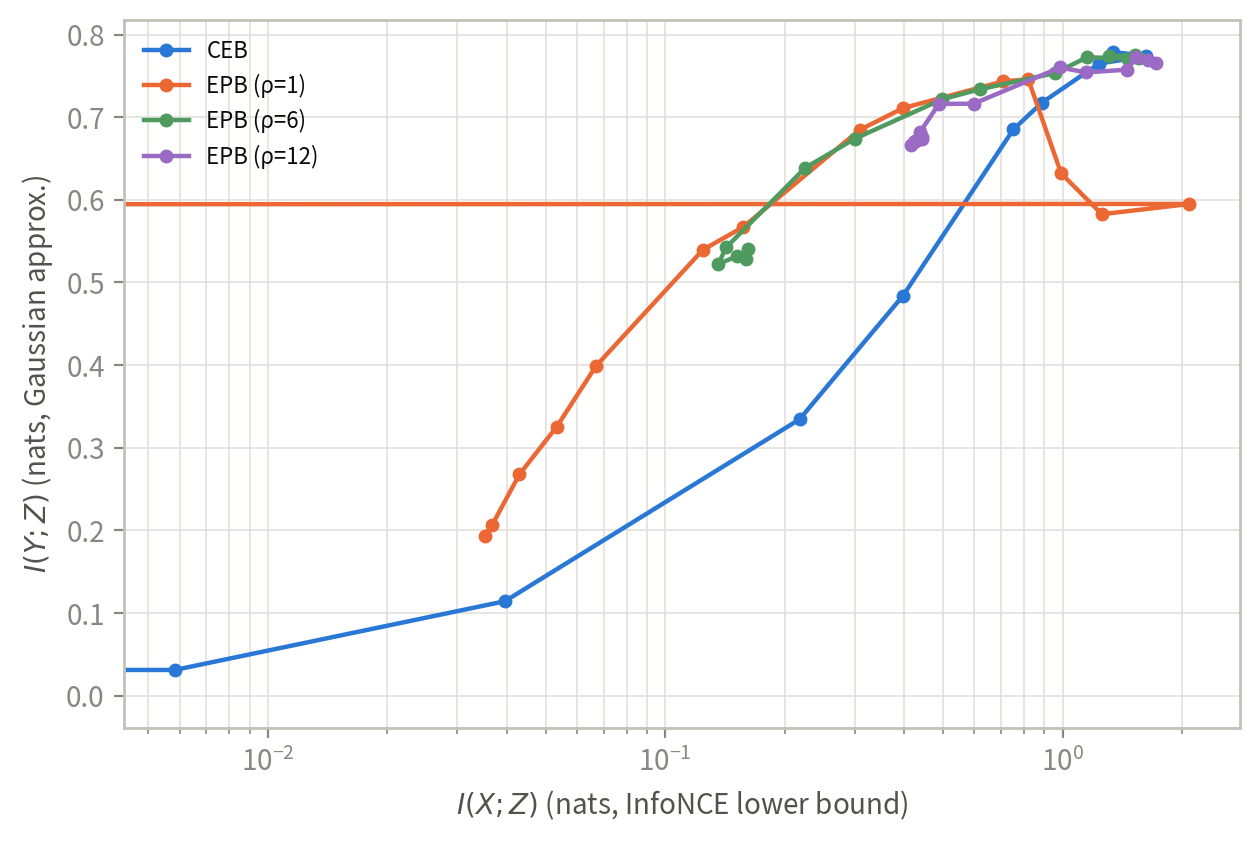
\includegraphics[width=0.48\linewidth]{figures/fig_info_plane_housing.png}\hfill
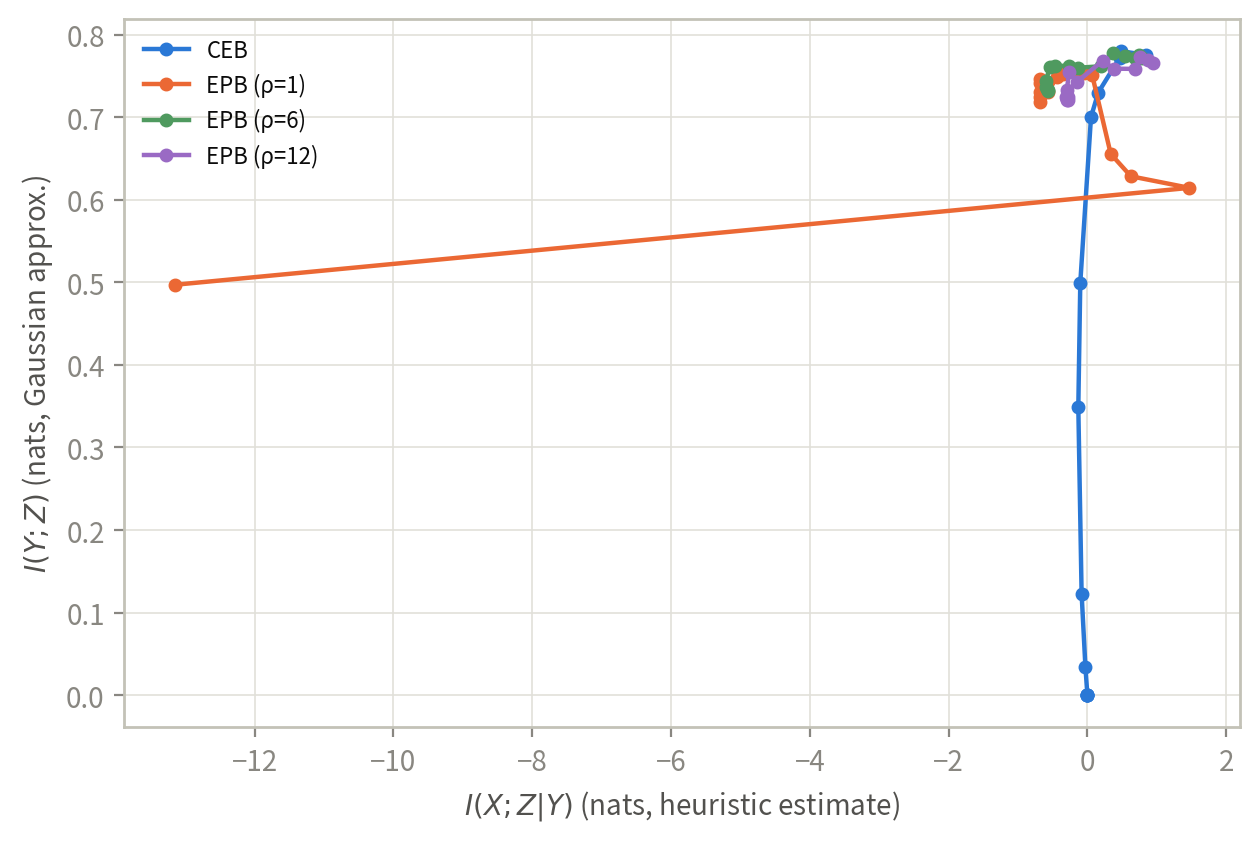
\includegraphics[width=0.48\linewidth]{figures/fig_certificate_plane_housing.png}
\caption{Information plane (a) and certificate plane (b) for Cal.~Housing,
companion panels to Fig.~\ref{fig:compression-main}(c,d): identical estimators,
$\beta$ grid (log $x$-scale in both panels), lines connect $\beta$ in
ascending order. CEB
one curve per panel; EPB three ($\rho \in \{1, 6, 12\}$).}
\label{fig:info-plane-extra}
\end{figure*}
